\documentclass[12pt, titlepage]{article}
\usepackage{cite}
\usepackage{amsbsy}
\usepackage[a4paper, total={6in, 8in}, left=40mm, top = 20mm, bottom = 20mm]{geometry}
\usepackage{graphicx}
\usepackage{multirow}
\usepackage{booktabs}
\usepackage{wasysym}
\usepackage{float}
\usepackage{setspace}
\usepackage[euler]{textgreek}
\usepackage{textcomp}
\usepackage{amssymb}
\usepackage{caption} 
\usepackage{lscape}
\captionsetup[table]{skip=10pt}
\doublespacing

\setlength{\parskip}{1em}
\setlength{\parindent}{4em}
\graphicspath{ {C:/Users/sra2g13/Documents/PhD/GitHub/mytophid-ears/Outputs/Graphs/} }
\title{Field metabolic rates of Scotia Sea myctophids (Family Myctophidae)\\
\large{Confirmation Report}}
\author{Sarah R. Alewijnse}     

\begin{document}
\maketitle
\tableofcontents
\pagebreak

\section{Abstract}

Myctophids (family Myctophidae) are an important part of the biological carbon pump in the oceans.
Estimating the magnitude of their contribution to the biological carbon pump requires knowledge of their field metabolic rate; the rate at which they use energy in the wild. %% NC: Is that technically true - isn't in the wild while going about normal activities? 
Currently, estimates of the resting metabolic rates of myctophids are based on a linear equation with log body mass and temperature as predictors.
Here, I estimated the field metabolic rate for six species of myctophid (\textit{Electrona antarctica, E. carlsbergi, Gymnoscopelus braueri, G. nicholsi, Protomyctophum bolini} and \textit{Krefftichthys anderssoni}) from the Scotia Sea, using a proxy for field metabolic rate based on otolith \textdelta \textsuperscript{13}C.
Estimates of resting metabolic rate did not correlate positively with estimates of field metabolic rate, contrary to expectations based on metabolic theories.
Additionally, differences among species were the most important drivers of variation in metabolic rate, rather log body mass and temperature.
% NC: Among is for > 2 things, between for 2 things
% NC: Is it worth being really explicit and ending this sentence with something like "as would be expected" or "as assumed in other studies"?
I explore why these differences may exist by examining the ecology and life history of the six species.
% NC: Instead maybe mention any implications?

\pagebreak
\section{Introduction}

Mesopelagic fishes (those living in the mesopelagic zone, between 150-1000m) are an important component of the ocean biological carbon pump. % cite various
They often undertake diel vertical migrations, swimming from depth to surface waters at night to feed on zooplankton, before returning to the deep prior to daybreak. % NC: I think avoid the abbreviation as it's just another thing to remember and doesn't cut out many words
By completing these migrations, migratory mesopelagic fishes transport carbon away from the surface waters, and export this carbon in the mesopelagic through respiration, excretion and mortality. 
Non-migratory mesopelagic fishes also contribute to the biological carbon pump by consuming migrating zooplankton in the mesopelagic zone. % Davidson
The deeper carbon is transported in the ocean, the longer it is prevented from returning to the surface and fluxing with the atmosphere. % https://www.int-res.com/articles/theme/m470p249.pdf
This carbon pump is at risk, however, as interest in harvesting mesopelagic fishes is increasing, driven by a growing requirement for fishmeal to sustain aquaculture. % Catul Davidson
To fully understand the impact of harvesting mesopelagic fishes, we must first quantify the role they play in the biological carbon pump.

Lanternfish (family Myctophidae) are the dominant mesopelagic fishes in the Scotia Sea, a highly productive area of the Southern Ocean. % Catul, Collins et al. 2012 (look for others) 
Scotia Sea myctophids are estimated to contribute 0.05 to 0.28 mg C m\textsuperscript{-2} d\textsuperscript{-1} to active carbon flux, equivalent to 9 to 47\% of gravitational particulate organic carbon flux in the same area, a substantial amount. % Belcher
This estimate is obtained from myctophid metabolic rate, which is calculated from the regression equation:

\begin{equation}
Ln(RMR_{M}) = a + b_{W} \times Ln(WM) + b_{T} \times T
\end{equation}

\noindent Where $RMR_{M}$ is wet mass-specific resting metabolic rate (\textmu l O\textsubscript{2} mg WM\textsuperscript{-1} h\textsuperscript{-1}), and $T$ is temperature (\textdegree C).
This equation was parameterised based five studies of myctophid respiration rate, so that $a$ = -1.315 \textpm 0.468, $b_{W}$ = -0.2665 \textpm 0.0516, and $b_{T}$ = 0.0848 \textpm 0.0108.
Studies used for parameterisation measured respiration rate through either respirometry or electron transport system enzyme activity (ETS). % Cite studies
Myctophids are delicate fishes, and are often dead or damaged on landing.
Consequently, fishes which are subjected to respirometry are likely to be stressed, giving an artificially high measure of metabolic rate.
Additionally, the most active fish in a catch are often selected for respirometry, which potentially biases measures towards fish with higher metabolic rates. % Torres & Somero
Respirometry measures the resting metabolic rate of a fish (RMR); the minimum metabolic rate of a resting organism, in a post-absorptive state. % Treberg
ETS measures the respiration potential of a sample of tissue, which is then converted to whole organism RMR using calibration curves of ETS and respirometry. % Azira, Ikeda & Cammen
A more useful measure of metabolic rate in the context of carbon modelling is field metabolic rate (FMR).

FMR is the time-averaged energy expenditure of an organism free-ranging in its natural habitat.
FMR includes energy expended on basal costs, as with RMR, but also incorporates the thermic effect of food (also called specific dynamic action), as well as energy used for growth, reproduction, movement and excretion. % Treberg Chung
As RMR is a component of FMR, studies predict that these two measures of metabolic rate will be positively correlated. % cite Degen & Kam etc
In this study, I used the stable isotopic composition of carbon (\textdelta \textsuperscript{13}C) in otoliths to calculate $M$, a proxy for FMR, % Chung & Trueman papers
for six species of myctophid common in the Scotia Sea. % Collins 2012, 2008 and Pusch et al. 2004
The aim of this study is to assess whether equation 1 is accurate in predicting FMR, by (1) comparing estimates of mass-specific metabolic rate generated from equation 1 to $M$; (2) investigating whether $M$ varies among species and (3) investigating whether $M$ can be predicted by linear models of log body mass (g) and temperature (\textdegree C), among and within species.

\pagebreak
\section{Methods} %NC: You flip back and forth between present and past tense below. I'd recommend making it all past tense.

\subsection{Data collection}

% Data needed
For analysis, I require estimates of $M$ and temperature, both of which are derived from otolith stable isotopes of carbon (\textdelta \textsuperscript{13}C) and oxygen (\textdelta \textsuperscript{18}O) respectively.
Otoliths are structures found within the inner ears of fishes,  made of calcium carbonate (usually aragonite) and an organic matrix. 
Otoliths grow sequentially, and once aragonite is laid down, it is metabolically inert.
This makes otoliths ideal structures for retrospectively acquiring FMR and temperature. % Campana, Chung
Otoliths from six species of myctophid from the Scotia Sea were donated by the British Antarctic Survey for this study: \textit{Electrona antarctica} (n = 19), \textit{E. carlsbergi} (n = 17), \textit{Gymnoscopelus braueri} (n = 20), \textit{G. nicholsi} (n = 13), \textit{Krefftichthys anderssoni} (n = 20) and \textit{Protomyctophum bolini} (n = 20).

Prior to stable isotope analysis, each otolith was cleaned in water, allowed to dry and mounted onto a backing plate (Struers EpoFix resin).
The outer surface of the otolith (100-200 \textmu m depth) was milled using an ESI NewWave Micromill, to ensure that the otolith material deposited most closely to the time of capture was analysed.
Where the otoliths were too small to be milled ($<$1mm diameter - all \textit{K. anderssoni} and some \textit{P. bolini}), they were crushed to obtain powder for stable isotope analysis.
Supplementary analyses (appendix X) were run to test whether this caused a significant difference in \textdelta \textsuperscript{13}C and \textdelta \textsuperscript{18}O.

% Isotopes
\textdelta \textsuperscript{13}C and \textdelta \textsuperscript{18}O of otolith aragonite were analysed using a Thermo Scientific Kiel IV Carbonate device, coupled with an MAT253 isotope ratio mass spectrometer.
Stable isotope values are expressed permil (\permil) % NC is it permil or per mille?
relative to Vienna Pee Dee Belemnite, according to the equation:

\begin{equation}
\delta X^{H} = \frac{R_{sample} - R_{standard}}{R_{standard}} \times 1000
\end{equation}

Where $X$ is the element, $^{H}$ is the mass of the heavy isotope of the element and $R$ is the ratio of the heavy to light isotope. % Fry

$M$ values are proportionalities % NC: Can you just say proportions? I've not come across this term before
of the percentage of metabolic carbon in a fish's blood, which is itself a proxy for mass-specific FMR.
The carbon in otolith aragonite is derived from this metabolic carbon, which is produced during cellular respiration and is itself derived from dietary carbon, and dissolved inorganic carbon, which is ingested from the surrounding seawater.
These two sources of carbon have isotopically distinct \textdelta \textsuperscript{13}C values, with \textdelta \textsuperscript{13}C from metabolic carbon being approximately 15$\permil$ higher than \textdelta \textsuperscript{13}C for dissolved inorganic carbon in most cases. % Chung 2019b
Based on this isotopic distinction, a mixing model can be used to estimate the proportion of metabolic carbon in the blood, $M$:

\begin{equation}
M = \frac{\delta^{13}C_{oto}-\delta^{13}C_{DIC-SW}}{\delta^{13}C_{diet}-\delta^{13}C_{DIC-SW}} + e_{total}
\end{equation}

\noindent Where $\delta^{13}C_{oto}$ is the \textdelta \textsuperscript{13}C value of the fish's otolith, $\delta^{13}C_{DIC-SW}$ is the value for \textdelta \textsuperscript{13}C of dissolved inorganic carbon (DIC) ingested by the fish through seawater, $\delta^{13}C_{diet}$ is the \textdelta \textsuperscript{13}C of the diet, and $e_{total}$ is the isotopic fractionation from DIC to blood, blood to endolymph, and endolymph to otolith. 
Where a fish has a higher FMR, it will produce more metabolic carbon, and thus have a higher $M$ value. 
For this study I assumed that $e_{total}$ was invariant across species, and that $M$ values were directly proportional to the percentage of metabolic carbon in the fish's blood.

In calculating $M$ values, parameters were allowed to vary across normal and truncated normal distributions with means, standard distributions, and minimum and maximum values set according to the relevant literature (appendix X). % set appendix number and cite each paper
$\delta^{13}C_{DIC-SW}$ was set using catch location and corrected for the Suess effect (the decrease in \textdelta \textsuperscript{13}C with time, due to anthropogenic carbon dioxide emissions), from the model by Tagliabue \& Bopp (2007).
$\delta^{13}C_{diet}$ was set using \textdelta \textsuperscript{13}C of phytoplankton (set by catch location) from the model by Magozzi \textit{et al.} 2017, trophic levels from FishBase % NC: cite
and the trophic enrichment factor for carbon from DeNiro \& Epstein (1978).
$e$ was set to the value from Solomon \textit{et al.} (2006).
10,000 random draws were sampled from the resulting distribution of $M$ values for each individual.

\textdelta \textsuperscript{18}O of otolith aragonite can be used to estimate the ambient temperature experienced by a fish. % Patterson et al. 1993, Thorrold et al. 1997, Hoie et al. 2004
Temperature was estimated using the following equation:

\begin{equation}
T = \frac{(\delta^{18}O_{oto} - \delta^{18}O_{SW}) - a}{b}
\end{equation}

\noindent Where $\delta^{18}O_{oto}$ is the \textdelta \textsuperscript{18}O of the otolith, $\delta^{18}O_{SW}$ is the \textdelta \textsuperscript{18}O of the ambient seawater, and a and b are parameters, set in this study according to H{\o}ie \textit{et al.} 2004. $\delta^{18}O_{SW}$  was set according to Schmidt \textit{et al.} 1999, by catch location and depth. 
As with $M$ values, all parameters were allowed to vary across normal and truncated normal distributions (appendix X). % set appendix number and cite each paper

\subsection{Statistical analyses}

All statistical analyses were carried out in R version 3.4.4. % NC: Cite R Core Team 2019
All Hamiltonian Monte Carlo (HMC) models were run in RStan version 2.17.3 % NC: cite
using the rethinking package version 1.59. % NC: cite
Convergence and mixing were checked using effective sample size (N\_eff), \^R, and traceplots (appendix X).

I generated estimates of log mass-specific RMR using equation 1, inputting body mass, and temperature calculated for \textdelta \textsuperscript{18}O.
The relationship between estimates of log mass-specific RMR and $M$ values was examined by using an HMC simulation of 10,000 iterations with 1000 warmup % NC: Is this the same as burnin? That's the more usual phrasing. What's the thinning interval? Same below.
and 4 chains.
The model equations were:

\begin{center}
$M \sim Normal(\mu, \sigma)$
\\$\mu = a + b \times Ln(RMR_{M})$
\\$a \sim Normal(0.2, 1)$
\\$b \sim Normal(0, 10)$
\\$\sigma \sim Cauchy(0.1, 1)$
\end{center}

To examine the effect of log body mass and temperature on $M$ values, I ran an HMC simulation of 1,000,000 iterations, with 500,000 warmup in a single chain. 
Species was included in the model as a random factor to address the problem of pseudoreplication. 
For brevity, this is referred to as the ``overall model''. 
The overall model was set as follows:

\begin{center}
$M \sim Normal(\mu, \sigma)$
\\$\mu = a_{1} + a\_Var_{Species} + b_{W} \times Ln(WM) + b_{T} \times T$
\\$a_{1} \sim Normal(0.20, 1)$
\\$b_{W} \sim Normal(0, 1)$
\\$b_{T} \sim Normal(0, 1)$
\\$a\_Var_{Species} \sim Normal(0, \sigma_{Species})$
\\$\sigma_{Species} \sim Cauchy(0, 1)$
\\$\sigma \sim Cauchy(0.1, 1)$
\end{center}

To examine the effect of log body mass and temperature on $M$ values within species, I ran HMC simulations of 10,000 iterations, with 1000 warmup, and 4 chains. 
Each model was set as follows:

\begin{center}
$M \sim Normal(\mu, \sigma)$
\\$\mu = a + a\_Var_{Species}$
\\$a \sim Normal(0.20, 1)$
\\$b_{W} \sim Normal(0, 1)$
\\$b_{T} \sim Normal(0, 1)$
\\$\sigma \sim Cauchy(0.1, 1)$
\end{center}

\pagebreak
Mean $M$ values for each species were also generated using an HMC simulation, with 10,000 iterations, 1000 warmup and 4 chains:

\begin{center}
$M \sim Normal(\mu, \sigma)$
\\$\mu = a + b_{W} \times Ln(WM) + b_{T} \times T$
\\$a\_Var_{Species} \sim Normal(0, \sigma_{Species})$
\\$\sigma_{Species} \sim Cauchy(0, 1)$
\\$\sigma \sim Cauchy(0.1, 1)$
\end{center}

\pagebreak
\section{Results}

\subsection{Comparison of estimates of metabolic rate}

$M$ values for myctophids decreased with increasing estimates of log mass-specific RMR ($a$ = 0.1682 \textpm 0.0072, $b$ = -0.0457 \textpm 0.0071, sigma = 0.0112 \textpm 0.0059, figure 1). 

% add posterior plots and precis

\begin{figure}[H]
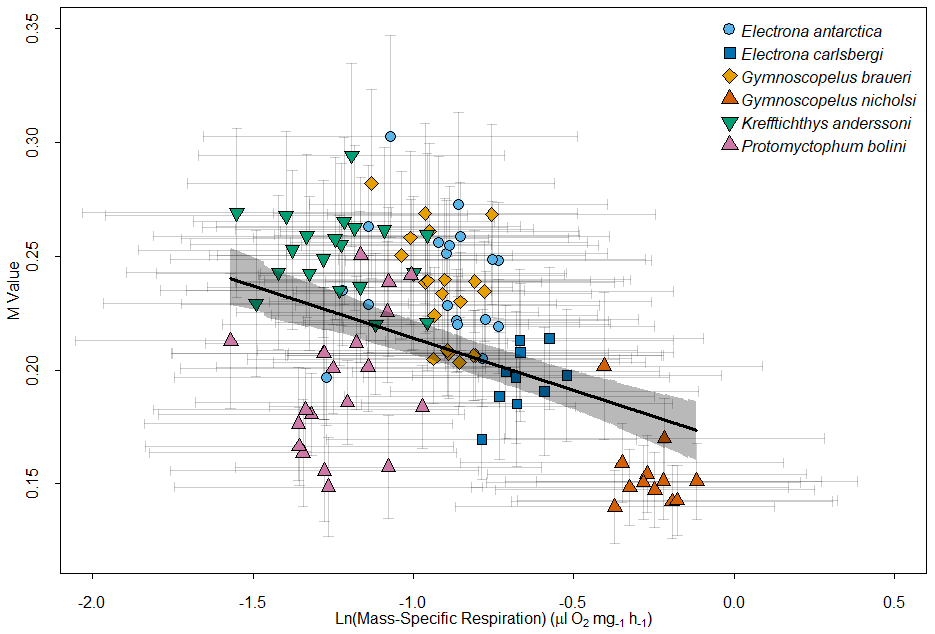
\includegraphics[width=\linewidth]{RMR_M.png}
\caption{Relationship between estimates of log mass-specific standard metabolic rate, derived from equation 1 and $M$ values, with standard deviation bars. Means (black line) and 89\% highest density posterior intervals (shaded) of posterior predictions are overlaid.} % cite belcher
\end{figure}

\pagebreak
\subsection{Scaling of $M$ values with body mass, temperature and species}

Neither log body mass nor temperature were correlated with $M$ values, as neither scaling exponent varied significantly from zero (figures 1 \& 2 and table 1).
Despite substantial overlap, the variable intercept of species was significantly greater than zero for \textit{K. anderssoni}, and significantly less than zero for \textit{G. nicholsi}, indicating that these species had higher and lower $M$ values respectively, compared to the other species.
\textit{K. anderssoni} ($M$ = 0.2459 \textpm 0.0227) \textit{E. antarctica} ($M$ = 0.2318 \textpm 0.0222) and \textit{G. braueri} ($M$ = 0.2252 \textpm 0.0223) had the highest species means of $M$, followed by \textit{E. carlsbergi} ($M$ = 0.1958 \textpm 0.0226) and \textit{P. bolini} ($M$ = 0.1875 \textpm 0.0222).
\textit{G. nicholsi} had the lowest estimates for $M$ ($M$ = 0.1526 \textpm 0.0222).
Supplementary analyses (appendix X) % set appendix number
provided no clear evidence that crushing whole otoliths, rather than milling, contributed to the lower \textdelta \textsuperscript{13}C in \textit{K. anderssoni}, and the resulting greater $M$ values for this species.

\begin{figure}[H]
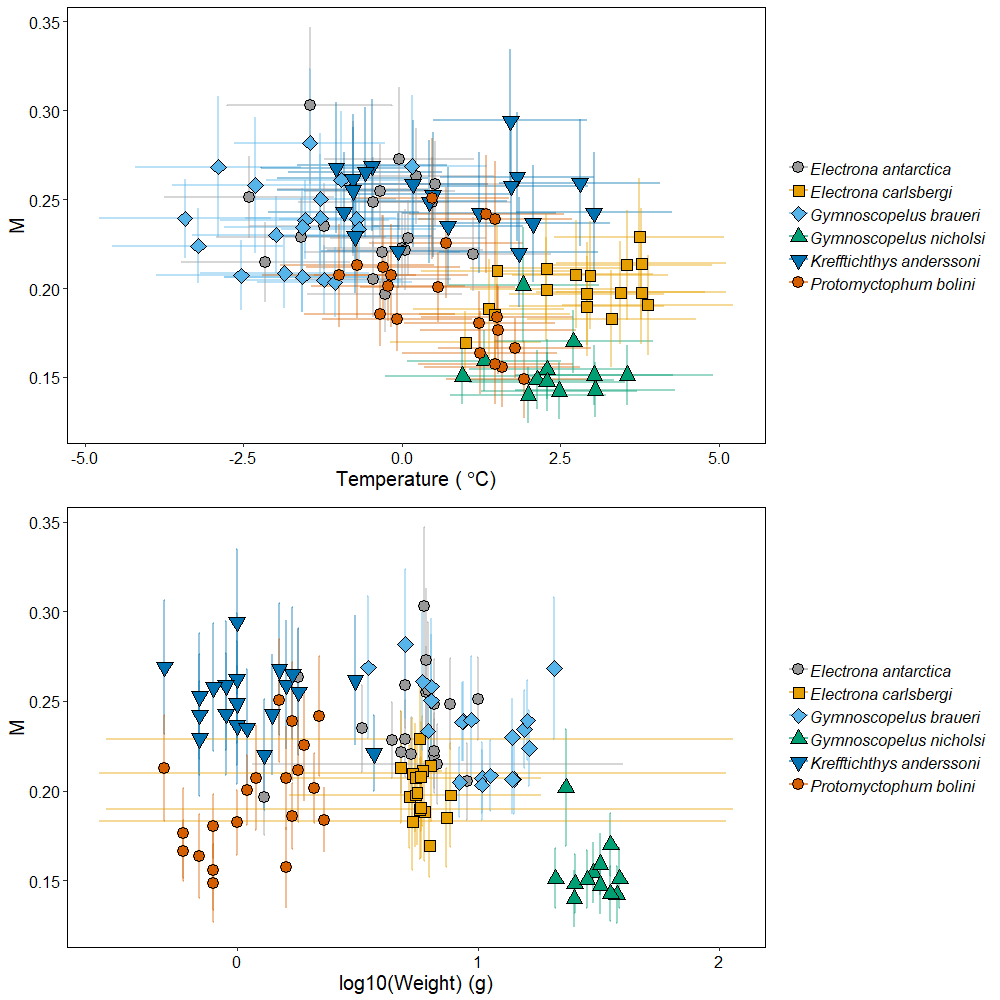
\includegraphics[width=\linewidth]{M_T_W.png}
\caption{Maximum density of distributions of $M$ values for individuals of six species of myctophid, with standard deviation bars, plotted against temperature (\textdegree C) in the top graph and log body mass (g) in the bottom graph. } %%
\end{figure}

\begin{figure}[H]
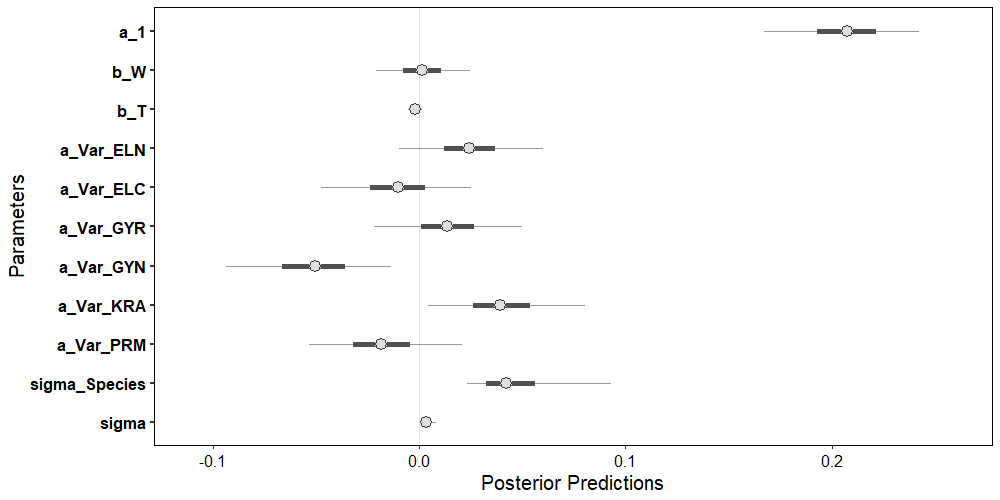
\includegraphics[width=\linewidth]{Params_Plot.png}
\caption{Plot of posterior predictions for model 1, showing maximum density posterior interval (dot), 50\% (thick line) and 90\% (thin line) highest density posterior intervals. ELN = \textit{Electrona antarctica}, ELC = \textit{E. carlsbergi}, GYR = \textit{Gymnoscopelus braueri}, GYN = \textit{G. nicholsi}, KRA = \textit{Krefftichthys anderssoni}, PRM = \textit{Protomyctophum bolini}.}
\end{figure}

\begin{table}
\begin{center}
\caption{Posterior predictions of parameters from the overall model, with convergence and mixing diagnostics: number of effective samples (N\_eff) and \^R. ELN = \textit{Electrona antarctica}, ELC = \textit{E. carlsbergi}, GYR = \textit{Gymnoscopelus braueri}, GYN = \textit{G. nicholsi}, KRA = \textit{Krefftichthys anderssoni}, PRM = \textit{Protomyctophum bolini}.}

\def\arraystretch{1.5}
  \begin{tabular}{ | l | l | l | l | l |}
    \hline
    \textbf{Parameter} & Mean & SD & N\_eff & \^R \\ \hline
    a\_1 & 0.2066 & 0.0244 & 12997 & 1.00 \\ \hline
    b\_W & 0.0015 & 0.0137 & 15468 & 1.00\\ \hline
    b\_T & -0.002 & 0.0022 & 14438 & 1.00 \\ \hline
    a\_Var\_ELN & 0.0246 & 0.0228 & 18448 & 1.00 \\ \hline
    a\_Var\_ELC & -0.0107 & 0.0237 & 11154 & 1.00 \\ \hline
    a\_Var\_GYR & 0.0135 & 0.0235 & 6617 & 1.00 \\ \hline
    a\_Var\_GYN & -0.0518 & 0.0257 & 14264 & 1.00 \\ \hline
    a\_Var\_KRA & 0.0402 & 0.0244 & 26605 & 1.00 \\ \hline
    a\_Var\_PRM & -0.0178 & 0.0241 & 7728 & 1.00 \\ \hline
    sigma\_Species & 0.0480 & 0.0254 & 59093 & 1.00 \\ \hline
    sigma & 0.0036 & 0.0024 & 1529 & 1.00 \\
    \hline
  \end{tabular}
  \end{center}
\end{table}

\begin{figure}[H]
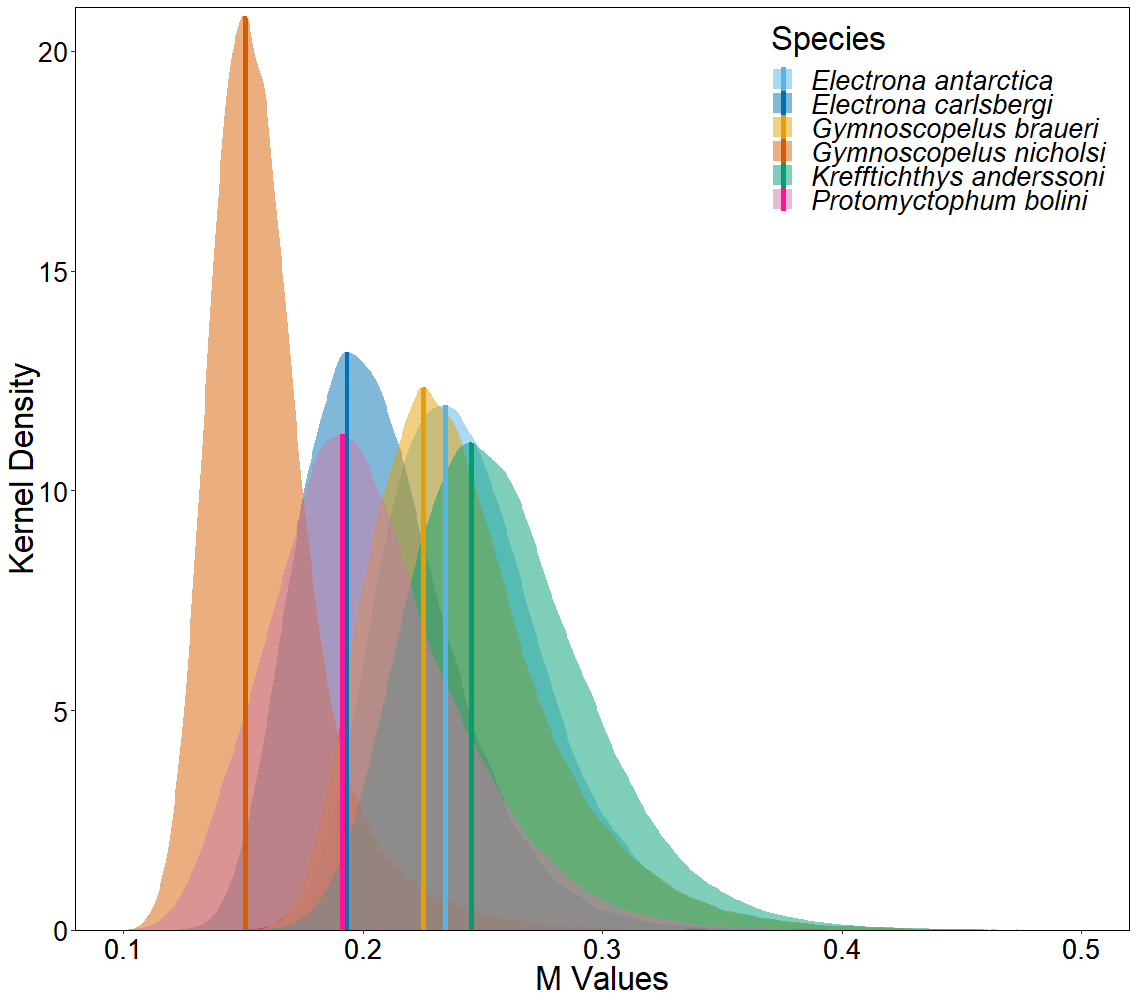
\includegraphics[width=\linewidth]{Density.png}
\caption{Kernel density plot of 10,000 estimates of $M$ (a proxy for FMR) per individual fish, across 108 individuals, combined and grouped by six species. Maximum density of the distribution of each species is indicated by the solid lines.}
\end{figure}

\pagebreak
\subsection{Within species variation in $M$ values}

Linear models of $M$ values with log body mass converged for \textit{E. antarctica, G. braueri} and \textit{P. bolini} (figure 5).
% NC: Maybe add : "Models for the other three species did not converge (I  will return to these models before publishing this paper)"
For \textit{E. antarctica} and \textit{G. braueri}, the scaling exponent was not significantly different from zero, suggesting that $M$ was invariant with log body mass in these species.
In \textit{P. bolini}, the scaling exponent was significantly greater than zero (b = 0.0257 \textpm 0.0118), indicating a that $M$ values increased with increasing log body mass.

\begin{figure}[H]
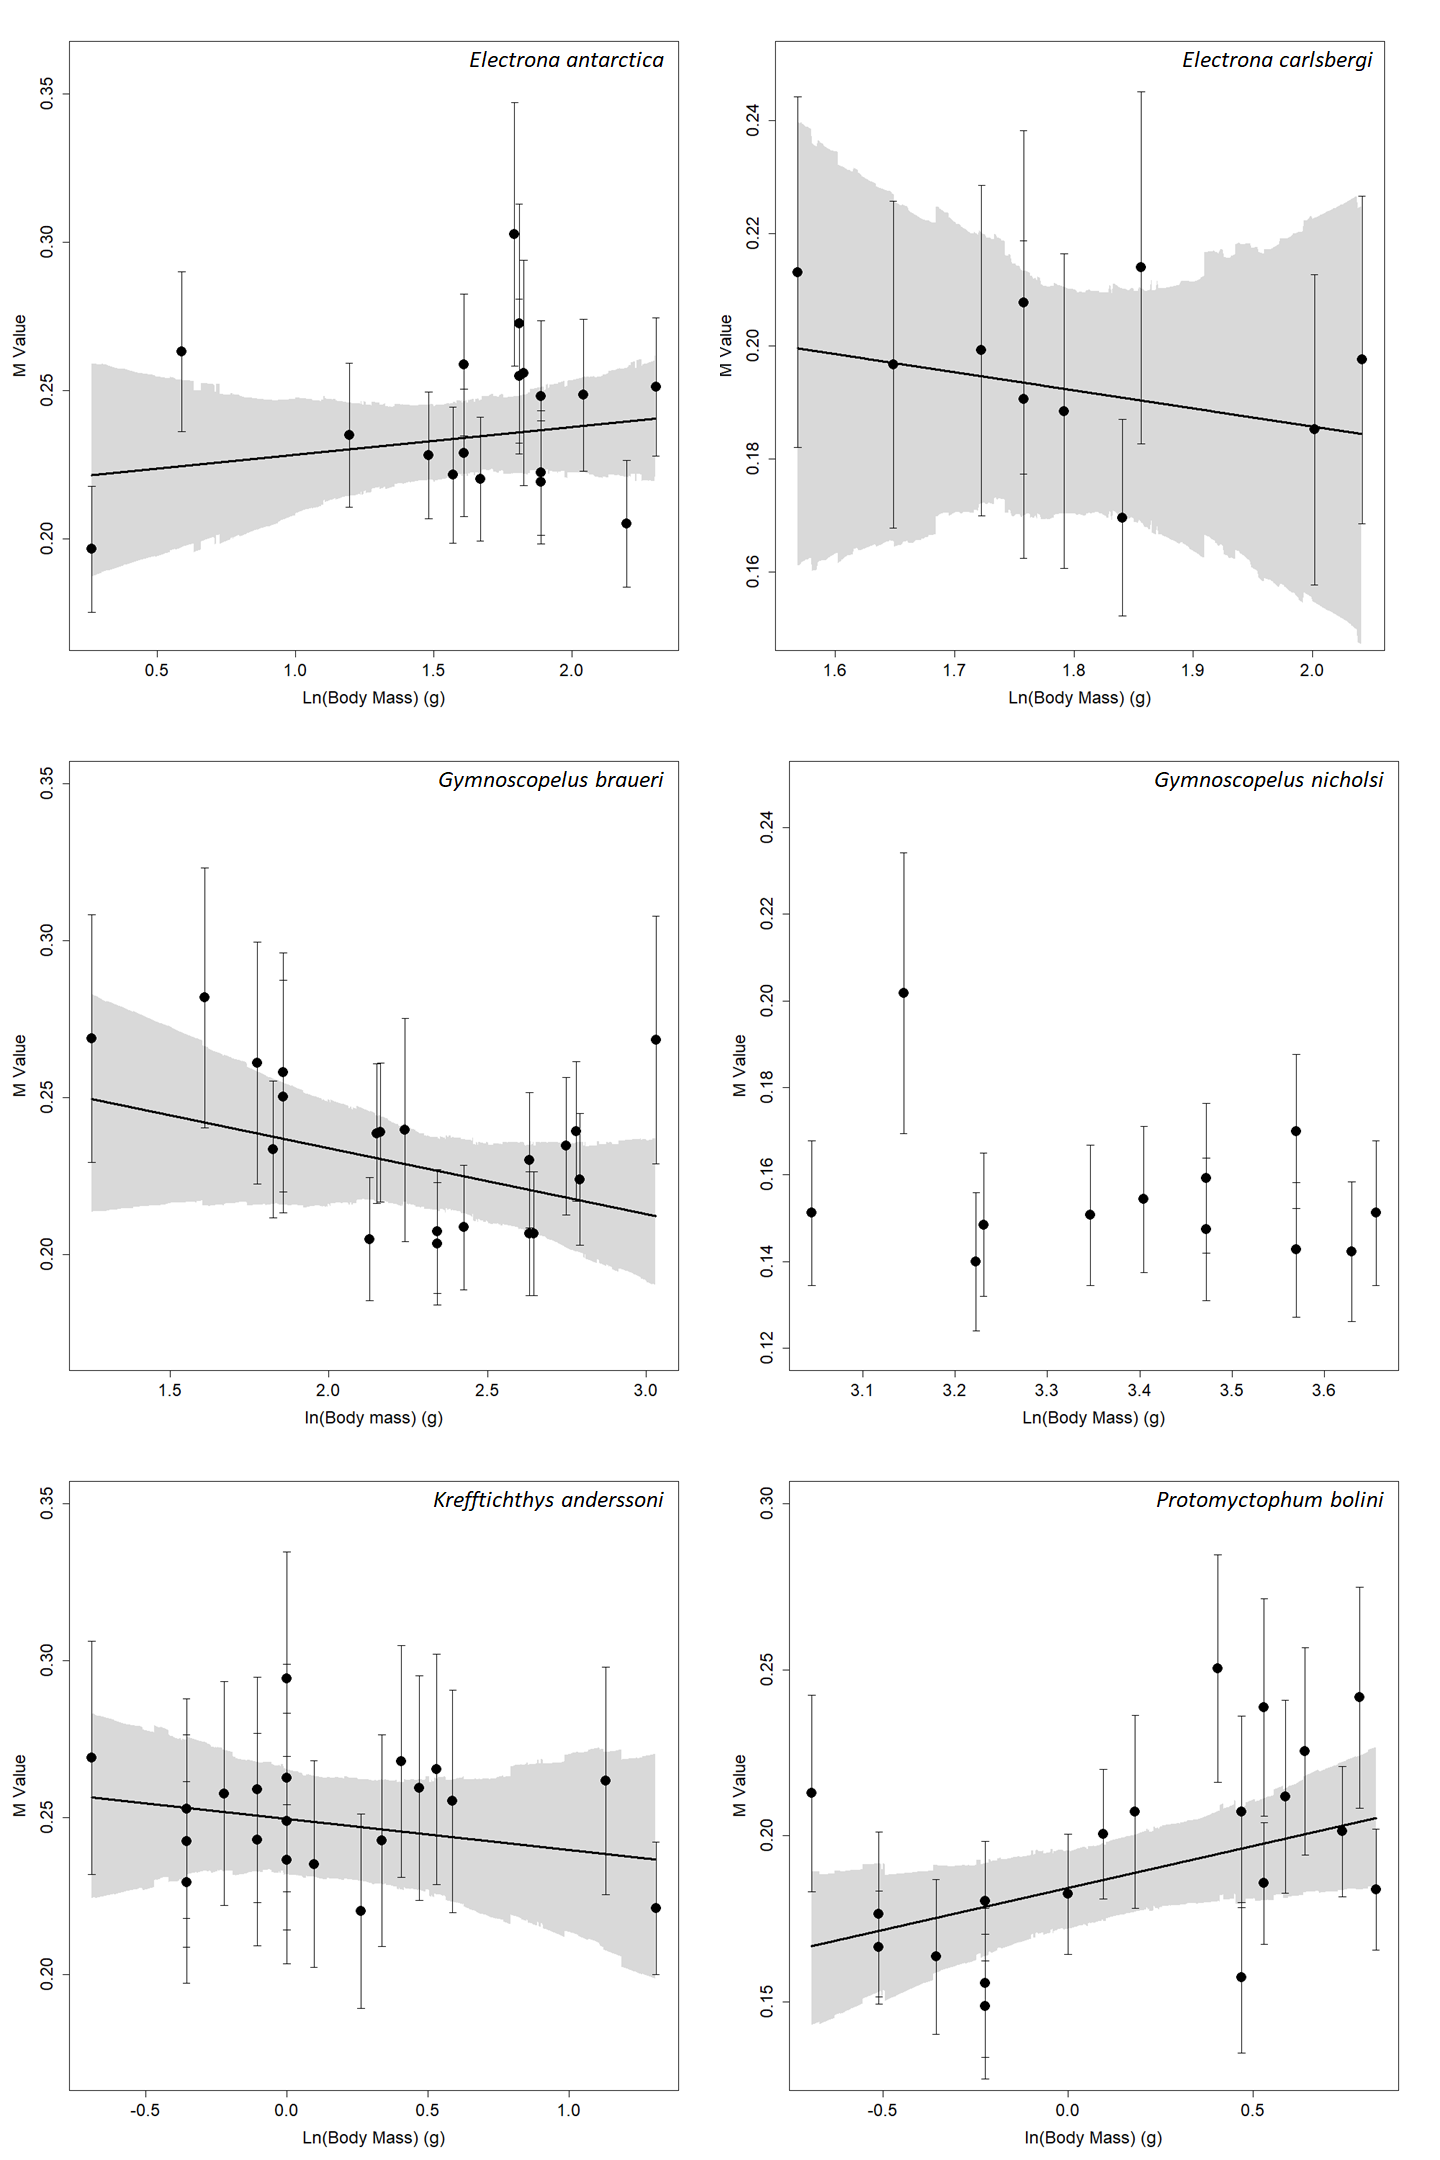
\includegraphics[width=\linewidth]{Combined_Weight.png}
\caption{Plots of log body mass (g) and $M$ values for each of the six species. Where linear models converged, they are plotted with the means (solid line) and 89\% highest density posterior interval (shaded areas).}
\end{figure}

Linear models of $M$ values and temperature converged for all species except for \textit{E. carlsbergi}.
In \textit{P. bolini}, the scaling exponent was significantly greater than zero (b = -0.0089 \textpm 0.0054), indicating a that $M$ values decreased with increasing temperature.

\begin{figure}[H]
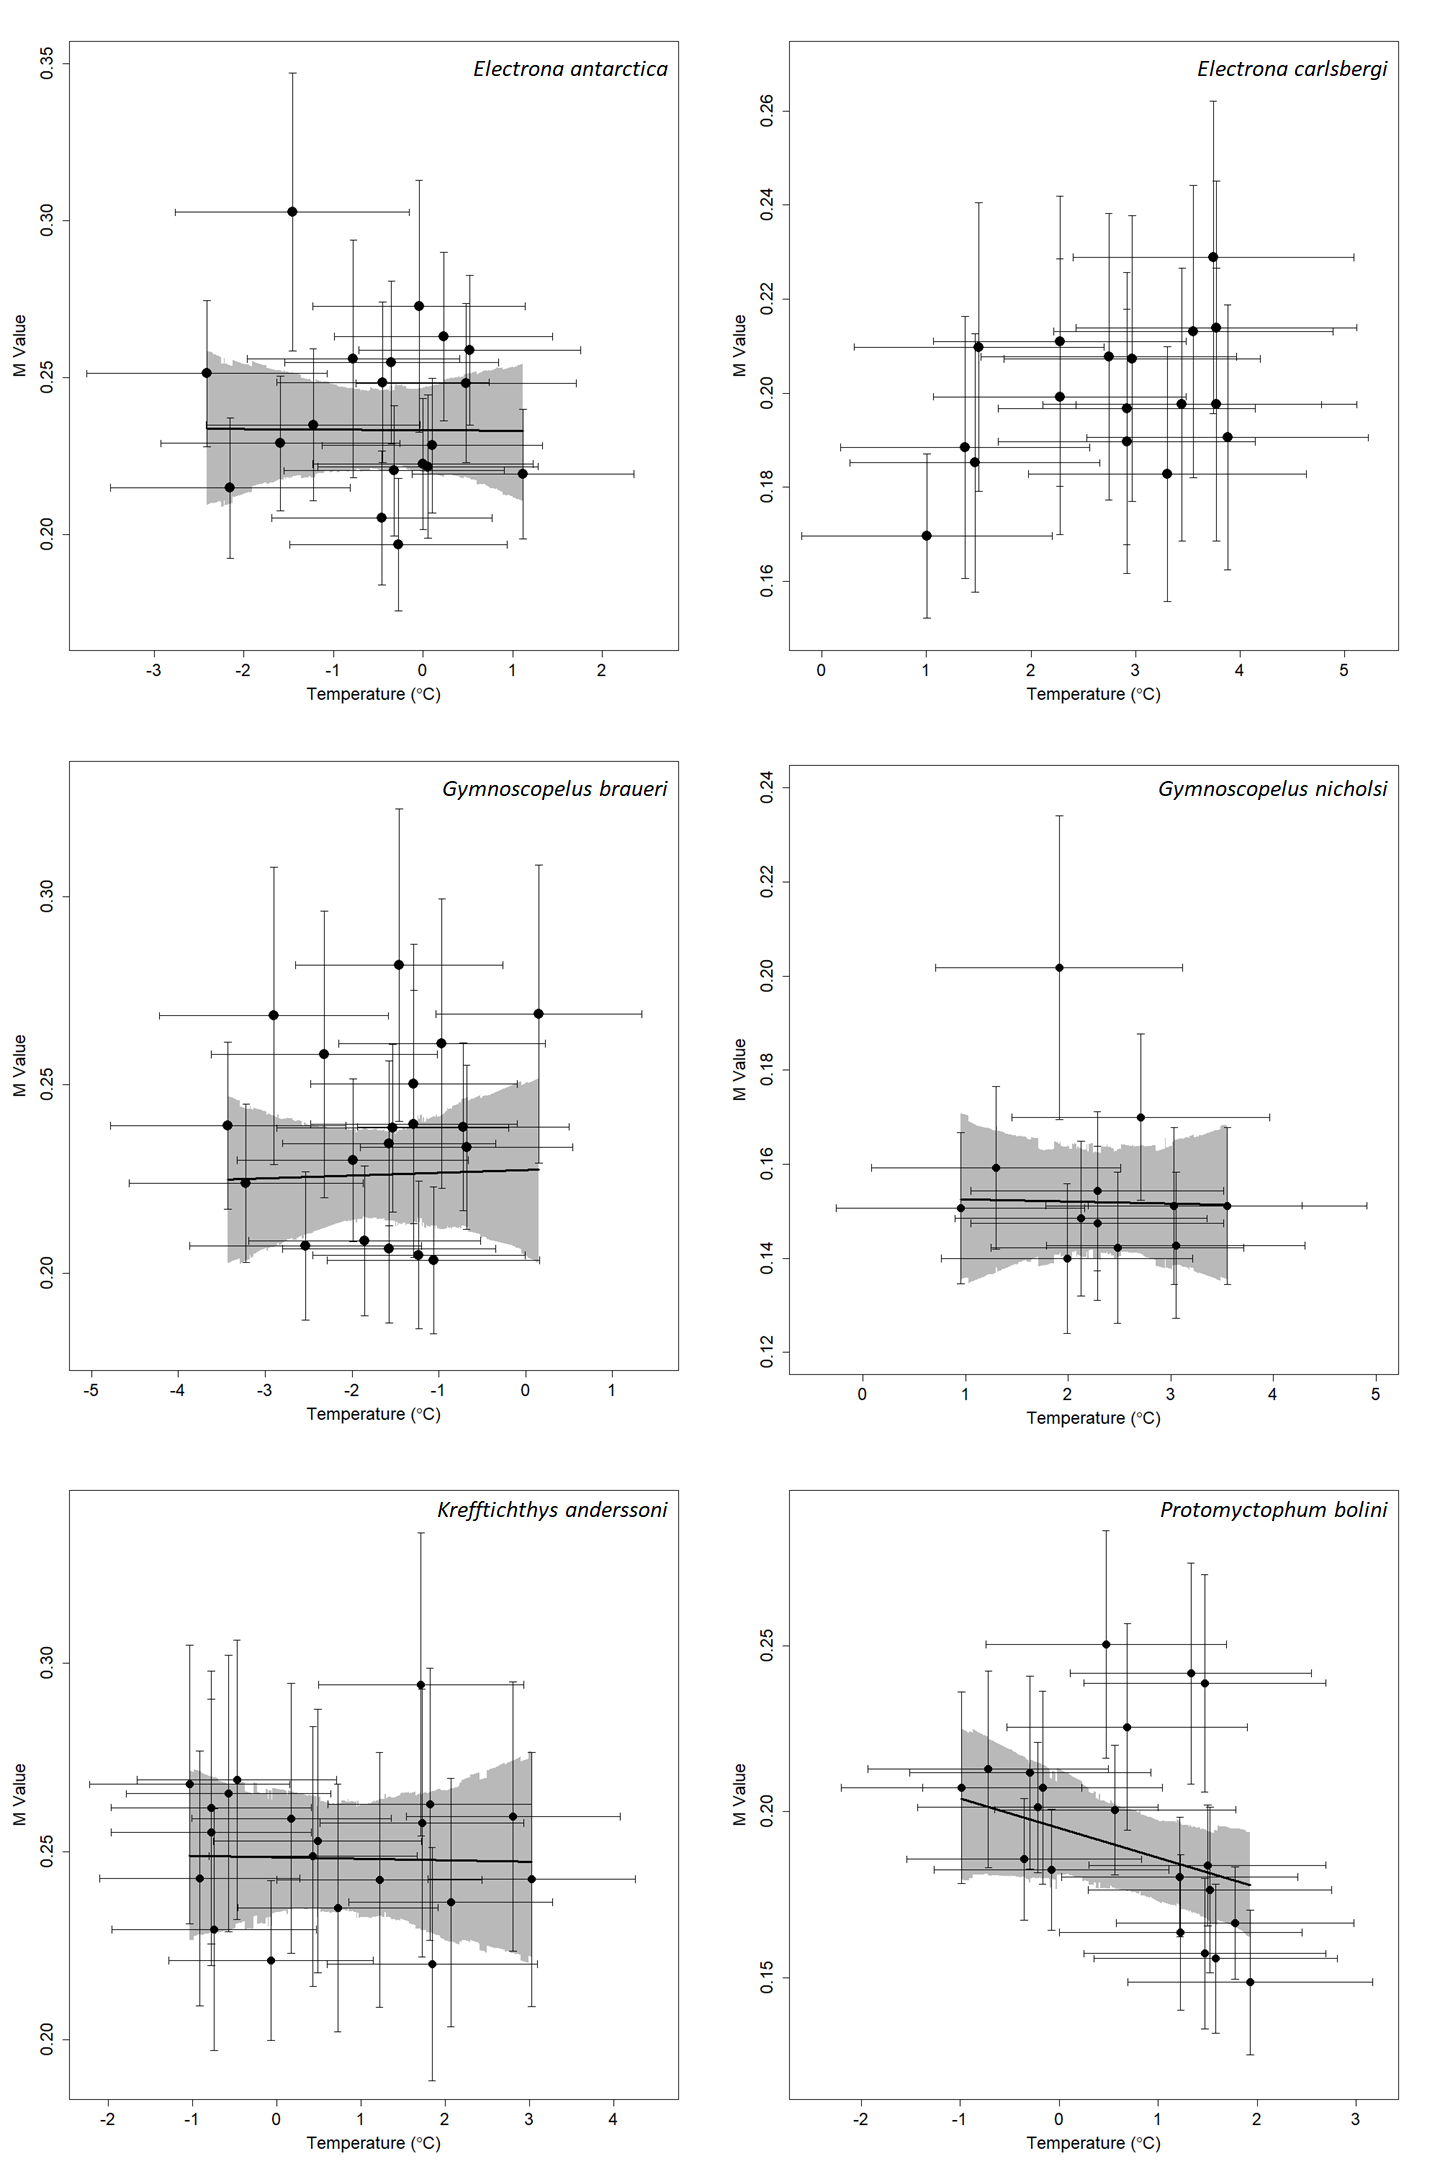
\includegraphics[width=\linewidth]{Combined_Temp.png}
\caption{Plots of log body mass (g) and $M$ values for each of the six species of myctophid. Where linear models converged, they are plotted with the means (solid line) and 89\% highest density posterior interval (shaded areas).}
\end{figure}

\pagebreak
\section{Discussion}

The negative linear relationship of $M$ values and log mass-specific resting metabolic rate (RMR) suggests that fishes with a high RMR have a low field metabolic rate (FMR), contrary to previous studies and metabolic theories. %NC: cite some?
%NC: I've defined RMR and FMR in this sentence just in case people have forgotten :). Be kind to the reader
Assuming that values of log mass-specific RMR are reasonable approximations (see discussion below), this suggests that the other components of FMR (thermic effect of food, growth, reproduction, movement and excretion) have a larger influence on FMR than RMR does.
These factors are more likely to be influenced by ecological differences among species, and this is supported by the result that species had the greatest influence on $M$ values.

While it is difficult to examine the effects of growth, reproduction, excretion, and the thermic effect of food, movement can be examined by comparing diel vertical migration strategies between species.
Different species of myctophid undertake diel vertical migrations to different degrees. % Watanabe et al. 1999 - Catul
\textit{K. anderssoni, E. antarctica} and \textit{G. braueri} are all known to perform these migrations year round.
These species also have a broad depth distribution, with individuals regularly found between 0-1000m depth.
Individuals of these species are undertaking daily or near daily migrations across a large depth range, increasing the amount of respiration attributable to movement.
This may account for the greater $M$ values seen in these species.
In contrast, there is no conclusive evidence for diel vertical migration in \textit{G. nicholsi, P. bolini}, and \textit{E. carlsbergi} undertakes migrations only in the summer.
Additionally, while individuals of these species are still occasionally found down to 1000m depth, the majority of the population stays above 700m in the case of \textit{G. nicholsi}, or above 400m for \textit{P. bolini} and \textit{E. carlsbergi}.
Given that these species are less likely to complete daily/near daily migrations, and if they do, are likely to be migrating across more compressed depth ranges, they are likely to have less respiration attributable to movement, which may explain their lower $M$ values.
Furthermore, there is evidence that \textit{G. nicholsi} individuals may become benthopelagic during late adulthood.
This would reduce their movement compared to pelagic fishes, resulting in a lower FMR, and could explain why this species has the lowest $M$ values of the six species in this study.

Throughout, I have assumed that the estimates of log mass-specific RMR from equation 1 are reasonable approximations of the true values, however there are issues with how the equation was parameterised.
Two of the studies used to parameterise equation 1 gave mass-specific RMR based on electron transport system activity (ETS).
ETS is converted to mass-specific RMR using ratios which varied between the two studies.
For example, one study used an ETS/RMR ratio of 2, % cite Ariza
while another used a ratio of 1.16. % cite Ikeda
The ETS/RMR ratio of 2 was used based on a study of zooplankton, % cite
while the ETS/RMR ratio of 1.16 was based on a study of gobies (family: Gobiidae) and pomacentrids (family: Pomacentridae). % cite
Uncertainty around the ETS/RMR ratio was not accounted for when calculating log mass-specific RMR from ETS, and consequently was not incorporated when parameterising equation 1.

Studies used to parameterise equation 1 had a much greater temperature range (0.5 to 20 \textdegree C) than was estimated for the fishes in our study (-3.4 to 3.9 \textdegree C, maximum density posterior values).
This may have overinflated the postive relationship between metabolic rate and temperature when comparing fishes from the relatively narrow range of temperatures in the Scotia Sea.

There was a slight negative relationship between temperature and $M$ values which may be an artefact of differing ecological factors between species.
Species with the lowest mean $M$ values (\textit{G. nicholsi}, \textit{P. bolini} and \textit{E. carlsbergi} are more common in the north of the Scotia Sea, % cite
where temperatures are warmer.
There is also evidence that these species do not complete their life cycles within the Scotia Sea, as the temperatures are too low for the more sensitive larval stages.
Recruitment for these species may occur outside of the Scotia Sea, with adults migrating in from elsewhere. % cite Saunders
This would mean that these species are living at the lowest end of their thermal range, which may inhibit their metabolic rates. % get references
In contrast, species with the highest mean $M$ values (\textit{K. anderssoni, E. antarctica} and \textit{G. braueri} are more common in the cooler, more southerly waters of the Scotia Sea.
These species are truly antarctic, with all life stages found in the Scotia Sea.
Individuals of these species are more likely to be living well within their thermal range, and therefore able to maintain higher metabolic rates, explaining the higher $M$ values.
More research on otoliths from individuals of \textit{G. nicholsi}, \textit{P. bolini} and \textit{E. carlsbergi} from sites north of the Scotia Sea would be needed to to confirm this theory. 
Given that temperature was not significantly correlated with $M$ values within any species, and that species captured the most variation in $M$ values, it seems likely that any negative correlation between species is an artefact.

Within species, log body mass and temperature were only significantly correlated with $M$ values in \textit{P. bolini}.
Within \textit{P. bolini}, $M$ values increased with increasing log body mass, and decreased with increasing temperature.
This is the opposite of what would be expected according to metabolic theory, and relationships of $M$ values with log body mass and temperature in previous studies, where mass-specific metabolic rate, and therefore $M$ values, decreased with increasing body mass, and increased with increasing temperature. % cite
The reason for this is unclear, and more measurements of $M$ values in this species, across a range of body masses, would be needed to investigate this further.

Without a calibration of $M$ values and mass-specific oxygen consumption for myctophids, equation 1 currently gives the best estimate of oxygen consumption for myctophids.
However, variation in $M$ values, and therefore FMR, is not adequately captured using log mass-specific RMR, log body mass or temperature as predictors.
Ecological factors such as migratory strategy are likely to be better predictors of FMR, but more research is needed across a wider range of species to confirm which ecological factors have the most influence on FMR.

\pagebreak
\section{Future Work}

This work will become one of the chapters in my thesis, and the first paper from my PhD.
When reworking this paper, I will make two main changes.

First, sensitivity analyses (appendix X) indicated that $\delta^{13}C_{diet}$ had the greatest influence on the final value of $M$. % Give appendix number
The \textdelta \textsuperscript{13}C value of muscle tissue, corrected for trophic fractionation factor, is a good approximation of the $\delta^{13}C_{diet}$ of an individual fish.
Each otolith used in this study also came with muscle tissue, which has been analysed for \textdelta \textsuperscript{13}C.
Unfortunately, the data were not available when this report was in preparation.
However, for the thesis chapter and paper manuscript, $M$ will be recalculated using this data, ensuring a more accurate and precise estimate for each fish.

Second, many HMC simulations in this study did not converge.
In future analyses, for my thesis chapter and when this is written into a paper, I will run HMC with a single, long chain, as opposed to four short chains, as was done with the overall model, and will try other modifications to ensure model convergence.

\pagebreak
\section{Thesis Plan and Gantt Chart}

\subsection{Overview of PhD}

The broad aim of my PhD is to investigate how the FMR of fishes varies at a macroecological scale. The work in this report forms the basis for one chapter of my PhD thesis. Aside from this and an introduction, I plan on three other chapters, outlined here.

\subsection{Chapters}

There are several theories as to how metabolic rate scales with body mass and temperature, and how it varies between species, including the metabolic theory of ecology and the metabolic level boundaries hypothesis.
These theories are used to predict how species might respond to climate change, and were initially developed using basal metabolic rate (BMR) data from endotherms, analogous to standard or resting metabolic rate (RMR) in ectotherms.
As discussed in the above report, field metabolic rate (FMR) is the more appropriate measure of metabolic rate in a modelling context.

There have been no studies examining how body mass and temperature scale with FMR in fishes. 
The common method for studying FMR in endotherms, the doubly-labelled water technique % cite lifson
does not work in fishes, due to their high water turnover rates. % cite from FProgRev
The otolith isotope technique for $M$ values, is ideal for investigating FMR at a macroecological scale, as otoliths archives are numerous, primarly due to their use in ageing fishes. %cite from FProgRev

I will first examine how $M$ values scale with log body mass and temperature.
This will form a chapter of my thesis, and a scientific paper.
I will then study which (if any) ecological factors influence $M$ values, based on previous studies of fish metabolic rates.
These ecological factors are habitat (benthic, benthopelagic or pelagic), % cite Killen papers
depth, % cite Somero Childress papers
body shape, % find refs
migratory habits and schooling or shoaling behaviours.
I will also investigate whether $M$ values correlated with growth, as estimated through the $k$ term in the von Bertalanffy growth equation.
I will use phylogenetic comparative methods to account for phylogenetic non-independence (the principle that species are not independent data points, due to their shared evolutionary history) % cite
and compare $M$ values across phylogenetic relationships.
This will inform the final chapter or chapters of my PhD, and related publications.

\subsection{Data Chapter}

Before undertaking the above studies, I need to build up a dataset of $M$ values from otolith isotope \textdelta \textsuperscript{13}C from a range of species of fishes across ecological categories and phylogeny.
The dataset currently consists of 42 species, with otoliths from a further 25 species awaiting stable isotope analysis.
Each species is represented by otoliths from ten individuals, and must have associated catch location and year, and a measure of body size.
The majority of the stable isotope analysis will take place in late 2019, when I visit the Life Sciences Mass Spectrometry Facility (figure 7) % Gantt chart
The dataset presently has good representation across benthopelagic (fishes living near seafloor) and deep-sea fishes, but is lacking in pelagic (fishes living in the water column away from the seafloor) and migratory fishes.
I am working on filling this gap by forming collaborations with other otolith researchers, and collecting otoliths from the Split fish market in Croatia.
Once other papers are published, we will publish this dataset as a data paper, to make it available to the wider scientific community.

\pagebreak
\begin{landscape}
\subsection{Gantt Chart}

\begin{figure}[H]
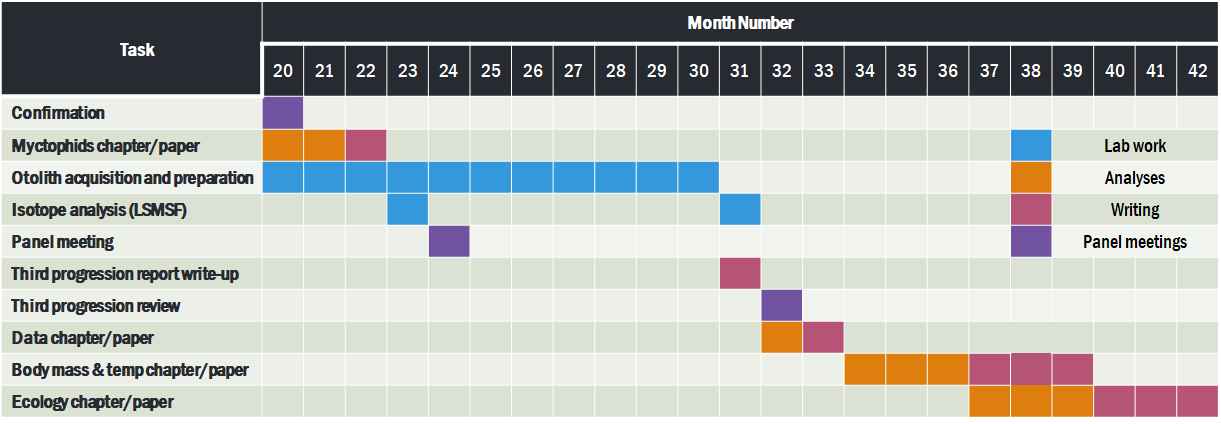
\includegraphics[width=\linewidth]{Gantt.png}
\caption{Gantt chart of expected progress until the end of my PhD.}
\end{figure}

\end{landscape}

\pagebreak
\section{Acknowledgements}

\end{document}

\begin{table}[H]
\begin{center}
\caption{Posterior predictions of parameters from the model of $M$ vs. ln(mass-specific respiration), with convergence and mixing diagnostics: number of effective samples (N\_eff) and \^R.}

\def\arraystretch{1.5}
  \begin{tabular}{ | l | l | l | l | l |}
    \hline
    \textbf{Parameter} & Mean & SD & N\_eff & \^R \\ \hline
    $a_{0}$ & 0.1682 & 0.0072 & 901 & 1.00 \\ \hline
    $a_{1}$ & -0.0457 & 0.0071 & 822 & 1.00 \\ \hline
    $\sigma$ & 0.0112 & 0.0059 & 244 & 1.01 \\
    \hline
  \end{tabular}
  \end{center}
\end{table} 